	
\documentclass[a4paper,12pt]{article} 
    \usepackage{amsmath, amssymb}
    \usepackage{kotex}
    \usepackage{graphicx}
    \usepackage[figuresright]{rotating} 
    
    \begin{document} 
    
    \title{과제7 보고서}
    \author{B211103 변준석}
    \date{2017년 10월}
    \maketitle

    \newpage
    \section{개요}
    이번 과제의 메인 프로그램인 \textsl{hw7.cpp} 에서는 연결리스트를 직접 구현하여 리스트 삽입, 제거 알고리즘을 구현하였다.
    
    \section{문제 해결 방안}
    연결리스트의 기본개념을 이해하고 \textsl{first}포인터와 \textsl{last}포인터를 이용하여 문제를 해결하였다.

    \section{\textsl{최종 출력}}
    \begin{figure}[t]\vspace*{4pt} 
    \centerline{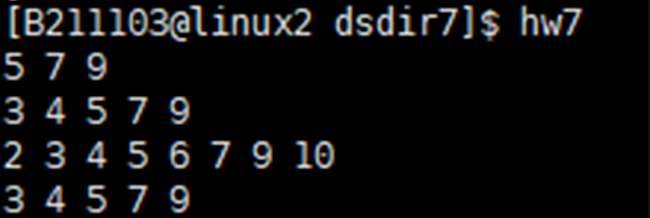
\includegraphics[width=1.0\columnwidth]{result}} 
    \caption{실행했을 때의 결과}\vspace*{-6pt} 
    \label{figure:result} 
    \end{figure} 
    
    
    \section{hw7의 간단한 설명}
    \textsl{PushBack}과 \textsl{PushFront}는 뒤/앞에 노드를 삽입하는 함수이며, \textsl{Insert}함수는 정렬되어있는 가정하에 제 위치에 삽입하는 함수이며, \textsl{Delete}는 리스트의 원소를 삭제하는 함수이다.
    \textsl{first}는 연결리스트의 첫 노드를 가르키는 포인터 변수이며, \textsl{last}는 마지막 노드를 가르키는 포인터 변수이다.

    
    \newpage
    \begin{figure}[t]\vspace*{4pt} 
    \centerline{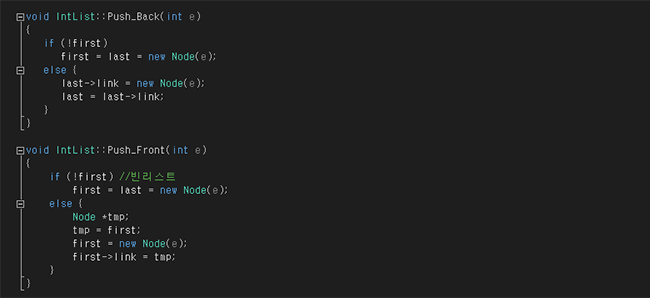
\includegraphics[width=1.0\columnwidth]{pbpf}} 
    \caption{list.cpp의 PushFront, PushBack함수}\vspace*{-6pt} 
    \label{figure:pbpf} 
    \end{figure} 
    
    \begin{figure}[t]\vspace*{4pt} 
    \centerline{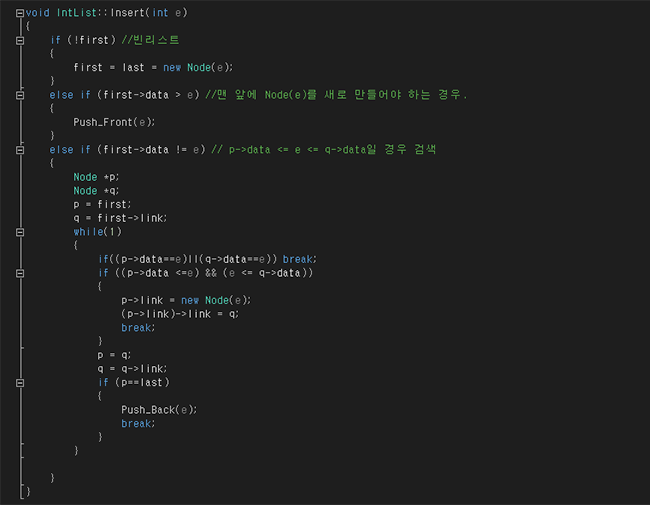
\includegraphics[width=1.0\columnwidth]{ins}} 
    \caption{list.cpp의 Insert함수}\vspace*{-6pt} 
    \label{figure:f2} 
    \end{figure} 
    
    \newpage
    \begin{figure}[t]\vspace*{4pt} 
    \centerline{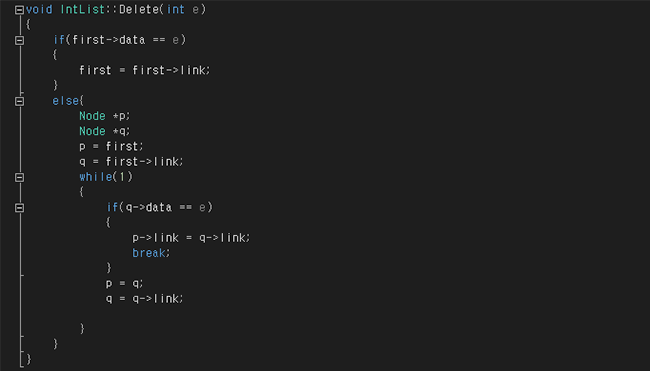
\includegraphics[width=1.0\columnwidth]{delete}} 
    \caption{list.cpp의 Delete함수}\vspace*{-6pt} 
    \label{figure:f3} 
    \end{figure} 
        
    \end{document}